%==========================================================================
% CAPÍTULO 5 — RESULTADOS PARCIAIS
%==========================================================================
\chapter{Resultados Parciais}
\label{chap:resultados}

\section{Nota Preliminar}

O presente capítulo reporta os resultados obtidos até à data de elaboração
deste relatório. Foram treinados três modelos progressivos sobre datasets
de complexidade crescente, todos utilizando a plataforma Roboflow Train
com o modelo base YOLO26 Nano. As contagens de imagens indicadas
referem-se sempre ao total após a aplicação de \textit{data augmentation}
pelo Roboflow.

\section{Métricas de Avaliação}

Para avaliar o desempenho dos modelos, são utilizadas as seguintes métricas
padrão na literatura de deteção de objetos:

\begin{description}
  \item[Precisão (P):] Fração das deteções positivas que são corretas.
    \[
      P = \frac{TP}{TP + FP}
    \]

  \item[Recall (R):] Fração dos objetos reais que foram detetados.
    \[
      R = \frac{TP}{TP + FN}
    \]

  \item[F1-Score:] Média harmónica entre Precisão e Recall.
    \[
      F1 = 2 \cdot \frac{P \cdot R}{P + R}
    \]

  \item[mAP@50:] \textit{Mean Average Precision} com limiar de IoU de 0,50.
    Métrica principal utilizada para comparação de modelos na literatura.

  \item[mAP@50-95:] Média do mAP calculado para limiares de IoU de 0,50
    a 0,95 (em passos de 0,05). Métrica mais exigente, adotada no COCO
    \textit{benchmark}.
\end{description}

\noindent onde $TP$ = Verdadeiros Positivos, $FP$ = Falsos Positivos,
$FN$ = Falsos Negativos.

% ------------------------------------------------------------------
\section{Resultados do Modelo 1 — \textit{Segmentation-Vineyard-2}}
% ------------------------------------------------------------------

O Modelo~1 foi treinado exclusivamente sobre as 300 imagens do
\textit{Segmentation-Vineyard-2} com as anotações de \textit{gomo}
adicionadas, resultando em aproximadamente 775 imagens após augmentation.
Este modelo serviu principalmente para validar a \textit{pipeline} técnica.
A inferência visual sobre imagens do conjunto de teste revelou que o modelo
identifica corretamente os sarmentos com elevada confiança (até 97\%) e os
troncos com boa confiança (acima de 83\%), validando a capacidade do
YOLO26 Nano de aprender a estrutura visual das videiras mesmo com datasets
de dimensão reduzida.

% ------------------------------------------------------------------
\section{Resultados do Modelo 2 — SVY-2 + Palmela}
% ------------------------------------------------------------------

A Tabela~\ref{tab:resultados_m2} apresenta as métricas obtidas pelo Modelo~2
no conjunto de validação, após treino sobre 772 imagens (augmentation de
400 imagens base: 300 do \textit{Segmentation-Vineyard-2} + 100 de Palmela).

\begin{table}[H]
  \centering
  \caption{Resultados do Modelo 2 (validação) — SVY-2 + Palmela, 772 imagens}
  \label{tab:resultados_m2}
  \begin{tabular}{lcccc}
    \toprule
    \textbf{Escopo}     & \textbf{P} & \textbf{R} & \textbf{F1} & \textbf{mAP@50} \\
    \midrule
    Todas as classes    & 54,3\%     & 52,7\%     & 53,5\%      & 48,8\%          \\
    \bottomrule
  \end{tabular}
\end{table}

\noindent\textit{Nota: O Roboflow Train, no plano gratuito, reporta apenas
métricas globais no painel principal. Os valores por classe estão disponíveis
nas ferramentas de avaliação avançada (plano pago).}

Um mAP@50 de 48,8\% é um resultado moderado mas coerente com as
condições do Modelo~2: dataset de domínio misto (espanhol + português),
quatro classes com densidades de instâncias muito distintas, e uma classe
(\textit{gomo}) completamente nova relativamente ao dataset base. A
precisão (54,3\%) e o recall (52,7\%) equilibrados indicam que o modelo
não está sistematicamente enviesado.

% ------------------------------------------------------------------
\section{Resultados do Modelo 3 — Dataset Expandido}
% ------------------------------------------------------------------

A Tabela~\ref{tab:resultados_m3} apresenta as métricas obtidas pelo Modelo~3,
treinado sobre 938 imagens (geradas por augmentation a partir das imagens
base disponíveis até 17 de junho de 2026).

\begin{table}[H]
  \centering
  \caption{Resultados do Modelo 3 (validação) — 938 imagens}
  \label{tab:resultados_m3}
  \begin{tabular}{lcccc}
    \toprule
    \textbf{Escopo}     & \textbf{P} & \textbf{R} & \textbf{F1} & \textbf{mAP@50} \\
    \midrule
    Todas as classes    & 57,3\%     & 40,5\%     & 47,4\%      & 43,7\%          \\
    \bottomrule
  \end{tabular}
\end{table}

A Figura~\ref{fig:resultado_m3_res} mostra uma inferência do Modelo~3 sobre
uma imagem das vinhas de Palmela, com \textit{confidence threshold} de 16\%.

\begin{figure}[H]
  \centering
  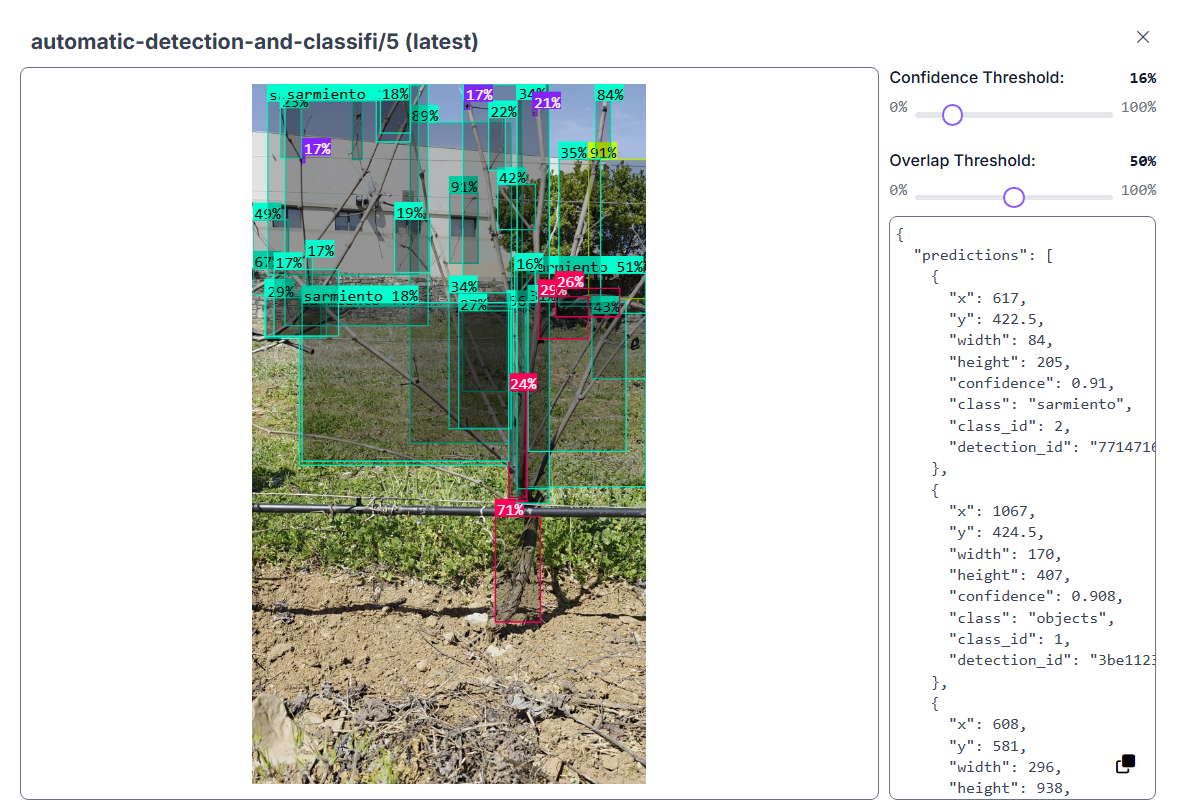
\includegraphics[width=0.80\textwidth]{imagens/resultado_v3.png}
  \caption{Inferência do Modelo~3 (threshold = 16\%). Os sarmentos (ciano)
           são detetados com confiança até 91\%; os gomos (roxo) surgem com
           confiança de 16--26\%; um obstáculo/poste é detetado a vermelho
           com 71\%.}
  \label{fig:resultado_m3_res}
\end{figure}

% ------------------------------------------------------------------
\section{Análise das Dificuldades Observadas}
% ------------------------------------------------------------------

A análise das inferências do Modelo~3 permite identificar três padrões
recorrentes de erro:

\begin{description}
  \item[Gomos com confiança insuficiente:] O modelo detecta a presença de
    gomos, mas a confiança atribuída (16--26\%) fica abaixo do limiar
    convencional de 50\%. Este padrão indica que a classe está a ser
    aprendida, mas o volume de dados de treino é ainda insuficiente para
    calibrar adequadamente a confiança.

  \item[Sarmentos de fundo confundidos com sarmentos de frente:]
    Em imagens com múltiplas videiras, sarmentos de segundo plano são
    por vezes detetados com alta confiança em detrimento dos de primeiro
    plano, pois têm maior contraste com o fundo.

  \item[Ausência de deteção de tronco em imagens de baixo contraste:]
    Em imagens com terreno de cor similar ao tronco, este não é detetado,
    apesar de estar visível.
\end{description}

% ------------------------------------------------------------------
\section{Comparação entre os Três Modelos}
% ------------------------------------------------------------------

A Tabela~\ref{tab:comparacao_modelos} resume as diferenças fundamentais
entre as três abordagens desenvolvidas neste estágio.

\begin{table}[H]
  \centering
  \caption{Comparação entre os três modelos desenvolvidos}
  \label{tab:comparacao_modelos}
  \begin{tabularx}{\textwidth}{l X X X}
    \toprule
    \textbf{Aspeto}          & \textbf{Modelo 1} & \textbf{Modelo 2} & \textbf{Modelo 3} \\
    \midrule
    Origem dos dados         & \textit{Segmentation-Vineyard-2} & SVY-2 + Palmela & SVY-2 + Palmela \\
    Imagens base             & $\approx$300      & $\approx$400      & $\approx$400+    \\
    Imagens (aug.)           & $\approx$775      & 772               & 938              \\
    N.º de classes           & 3                 & 4                 & 4                \\
    Complexidade das imagens & Moderada          & Alta              & Alta             \\
    Aplicabilidade real      & Limitada          & Alta              & Alta             \\
    mAP@50                   & ---               & 48,8\%            & 43,7\%           \\
    Precisão                 & ---               & 54,3\%            & 57,3\%           \\
    Recall                   & ---               & 52,7\%            & 40,5\%           \\
    F1                       & ---               & 53,5\%            & 47,4\%           \\
    Estado                   & Concluído         & Concluído         & Ativo            \\
    \bottomrule
  \end{tabularx}
\end{table}

A transição do Modelo~2 para o Modelo~3 evidencia um padrão coerente com
o aumento da dificuldade do dataset: o mAP@50 desce de 48,8\% para 43,7\%,
mas a Precisão sobe de 54,3\% para 57,3\% (menos falsos positivos). A
queda no Recall de 52,7\% para 40,5\% reflete principalmente a dificuldade
de detetar gomos com confiança suficiente nas novas imagens de Palmela,
mais complexas e variadas.
